\documentclass[12pt, letterpaper]{article}

\usepackage[english]{babel} % Sets the language and regional settings for English documents
\usepackage[utf8]{inputenc} % Allows the use of UTF-8 characters in the document
\usepackage[T1]{fontenc} % Specifies the font encoding
\usepackage[margin=2cm]{geometry} % Sets the page margins
\usepackage{makeidx} % Enables the creation of indexes
\usepackage{natbib} % Provides flexible bibliography support
\usepackage{url} % Allows the use of URLs
\usepackage{enumitem} % Customizes the appearance of lists
\usepackage{listings} % Provides syntax highlighting for code listings
\usepackage[dvipsnames]{xcolor} % Allows the use of colors
\usepackage{parskip} % Modifies paragraph spacing
\usepackage{graphicx} % Enables the inclusion of graphics
\usepackage{tikz} % Allows the creation of graphics and diagrams
\usepackage{float} % Provides improved control over the placement of figures and tables
\usepackage{hyperref} % Enables the creation of hyperlinks
\usepackage{amsmath} % Provides additional math environments and commands
\usepackage{circuitikz} % Allows the creation of electrical circuits
\usepackage{adjustbox} % Adjusts the size of the circuit diagrams
\usepackage{arydshln} % Allows the use of dashed lines in tables
\usepackage{tcolorbox}

\usetikzlibrary{shapes.geometric, positioning}
\definecolor{mygray}{gray}{0.9}

\lstset{
	language=SQL,
	basicstyle=\ttfamily\small,
	keywordstyle=\color{blue},
	commentstyle=\color[rgb]{0,0.5,0},
	stringstyle=\color{red},
	numbers=left,
	numberstyle=\tiny\color{gray},
	stepnumber=1,
	numbersep=10pt,
	backgroundcolor=\color{white},
	showspaces=false,
	showstringspaces=false,
	breaklines=true,
	frame=single,
	tabsize=2, captionpos=b, lineskip=-1pt,
	extendedchars=true,
	literate={á}{{\'a}}1 {é}{{\'e}}1 {í}{{\'i}}1 {ó}{{\'o}}1 {ú}{{\'u}}1 {Á}{{\'A}}1 {É}{{\'E}}1 {Í}{{\'I}}1 {Ó}{{\'O}}1 {Ú}{{\'U}}1 {ñ}{{\~n}}1 {Ñ}{{\~N}}1 {¿}{{\textquestiondown}}1 {¡}{{\textexclamdown}}1
}

% VHDL language configuration
\lstdefinelanguage{VHDL}{
	morekeywords={entity, architecture, signal, port, in, out, inout, begin, end, process, if, then, else, elsif, case, when, others, for, while, loop, wait, library, use, std_logic, std_logic_vector, integer, boolean, rising_edge, falling_edge, component, generic, map, downto, to, and, or, not, xor, nand, nor, xnor},
	morecomment=[l]{--},
	morestring=[b]",
	sensitive=false,
	alsoletter={_}
}

% VHDL listings style
\lstdefinestyle{vhdl}{
	language=VHDL,
	basicstyle=\ttfamily\small,
	keywordstyle=\color{blue}\bfseries,
	commentstyle=\color[rgb]{0,0.6,0}\itshape,
	stringstyle=\color{red},
	numbers=left,
	numberstyle=\tiny\color{gray},
	stepnumber=1,
	numbersep=10pt,
	backgroundcolor=\color{white},
	showspaces=false,
	showstringspaces=false,
	breaklines=true,
	frame=single,
	tabsize=2,
	captionpos=b,
	lineskip=-1pt,
	extendedchars=true
}

\graphicspath{ {./img/} } % Sets the path for the graphics

\newlist{biblio}{enumerate}{1}
\setlist[biblio,1]{label=[\arabic*]}

\makeindex

\begin{document}

\begin{titlepage}

	\begin{tikzpicture}[remember picture,overlay]
		\node[anchor=north west, inner sep=30] at (current page.north west) {
			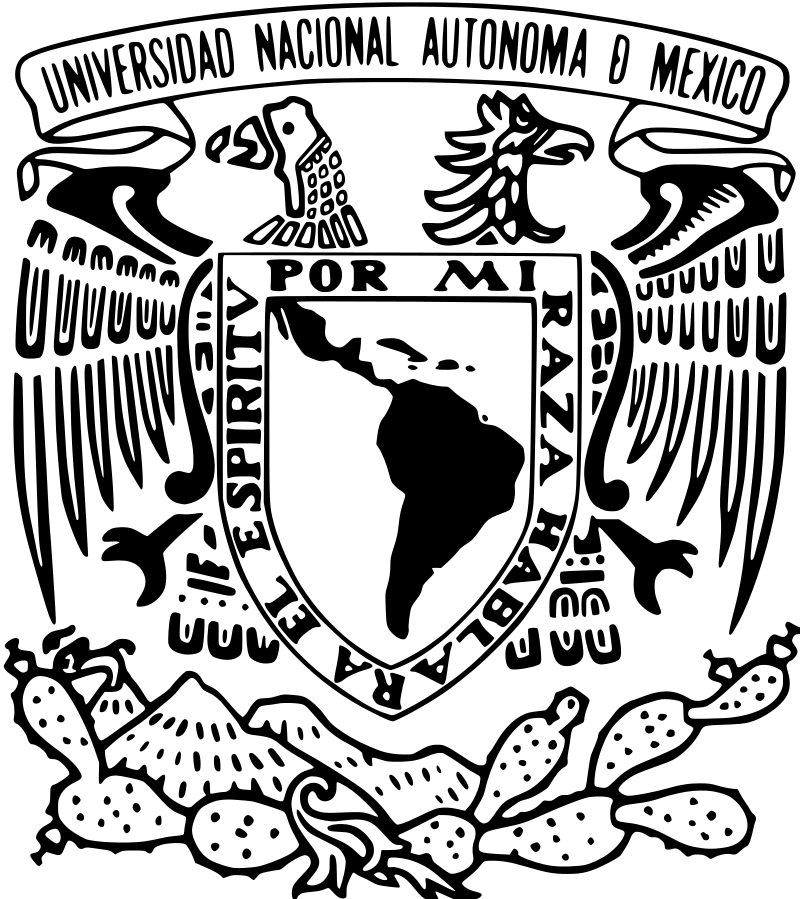
\includegraphics[width=4cm]{escudoUNAM.png}
		};

		\node[anchor=north east, inner sep=30] at (current page.north east) {
			
\includegraphics[width=4cm]{escudoFI.png}
		};
	\end{tikzpicture}

	\begin{center}
		\vspace*{3cm}

		\Huge
		\textbf{Práctica 1 - Análisis Senoidal Permanente de Circuitos Lineales}

		\vspace{2.5cm}

		\Huge
		\textbf{Facultad de Ingeniería}\\
		Circuitos Eléctricos\\
		Semestre 2026-1\\

		\vspace{2.5cm}

		\textbf{Grupo:} 4

		\vspace{2.5cm}

		\Huge
		Ugartechea González Luis Antonio\\
		Tepal Brinseño Hansel Yael\\
		\textbf{Fecha de entrega:} 30 de septiembre de 2025
		\vspace{2.5cm}
	\end{center}

\end{titlepage}

\section{Objetivo}

\begin{itemize}
	\item Verificar en forma práctica las técnicas de análisis senoidal permanente, empleando fasores.
\end{itemize}

\section{Introducción}

En el análisis de circuitos eléctricos, es fundamental comprender los conceptos de fasores y funciones de transferencia, ya que permiten simplificar y modelar el comportamiento de sistemas lineales ante señales sinusoidales. El uso de fasores facilita la representación compleja de magnitudes sinusoidales, mientras que la función de transferencia describe la relación entre la entrada y la salida de un sistema en el dominio de Laplace, bajo condiciones iniciales nulas.

\section{Desarrollo}

\subsection*{Experimento 1. Circuito RL}

\begin{figure}[H]
	\centering
	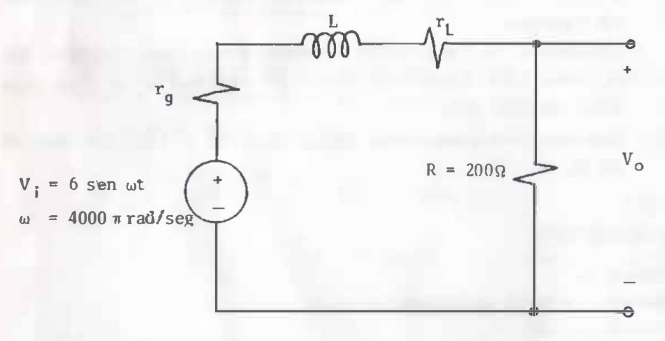
\includegraphics[width=0.5\textwidth]{figure_1.png}
	\caption{Circuito RL}
\end{figure}

\subsubsection*{Función de Transferencia}

\[H(s) = \frac{R}{R_{eq} + sL}\]

\[H(j\omega) = \frac{R}{R_{eq} + j\omega L}\]

\subsubsection*{Obtención de ángulo de fase}

\[\Theta_Y = \angle Y(j\omega)\]

\[\Theta_X = \angle X(j\omega)\]

\[\Theta_Y = \tan^{-1}\left(\frac{\text{Im}(Y(j\omega))}{\text{Re}(Y(j\omega))}\right)\]

\[\Theta_X = \tan^{-1}\left(\frac{\text{Im}(X(j\omega))}{\text{Re}(X(j\omega))}\right)\]

\[\Theta_Y = \tan^{-1}\left(\frac{0}{R}\right)\]

\[\Theta_X = \tan^{-1}\left(\frac{\omega L}{R_{eq}}\right)\]

\[\Theta_H = \Theta_Y - \Theta_X\]

\subsubsection*{Magnitud de la señal}

\[
|H(j\omega)| = \frac{R}{\sqrt{R_{eq}^2 + (\omega L)^2}}
\]

\subsubsection*{Datos de Practica}

\begin{itemize}
	\item \textbf{Señal de entrada:} \(5 sen (\omega t)\)
	\item \textbf{\(\omega\):} \(4000 \pi \, rad/s\)
	\item \textbf{Frecuencia:} \(f = 2 kHz\)
	\item \textbf{Resistencia de la fuente:} \(50 \Omega\)
	\item \textbf{Inductancia:} \(L =  72 mH\)
	\item \textbf{resistencia del inductor:} \(R_L = 72.7 \Omega\)
	\item \textbf{Resistencia:} \(R = 200 \Omega\)
\end{itemize}

\subsection*{Osciloscopio}

\begin{figure}[H]
	\centering
	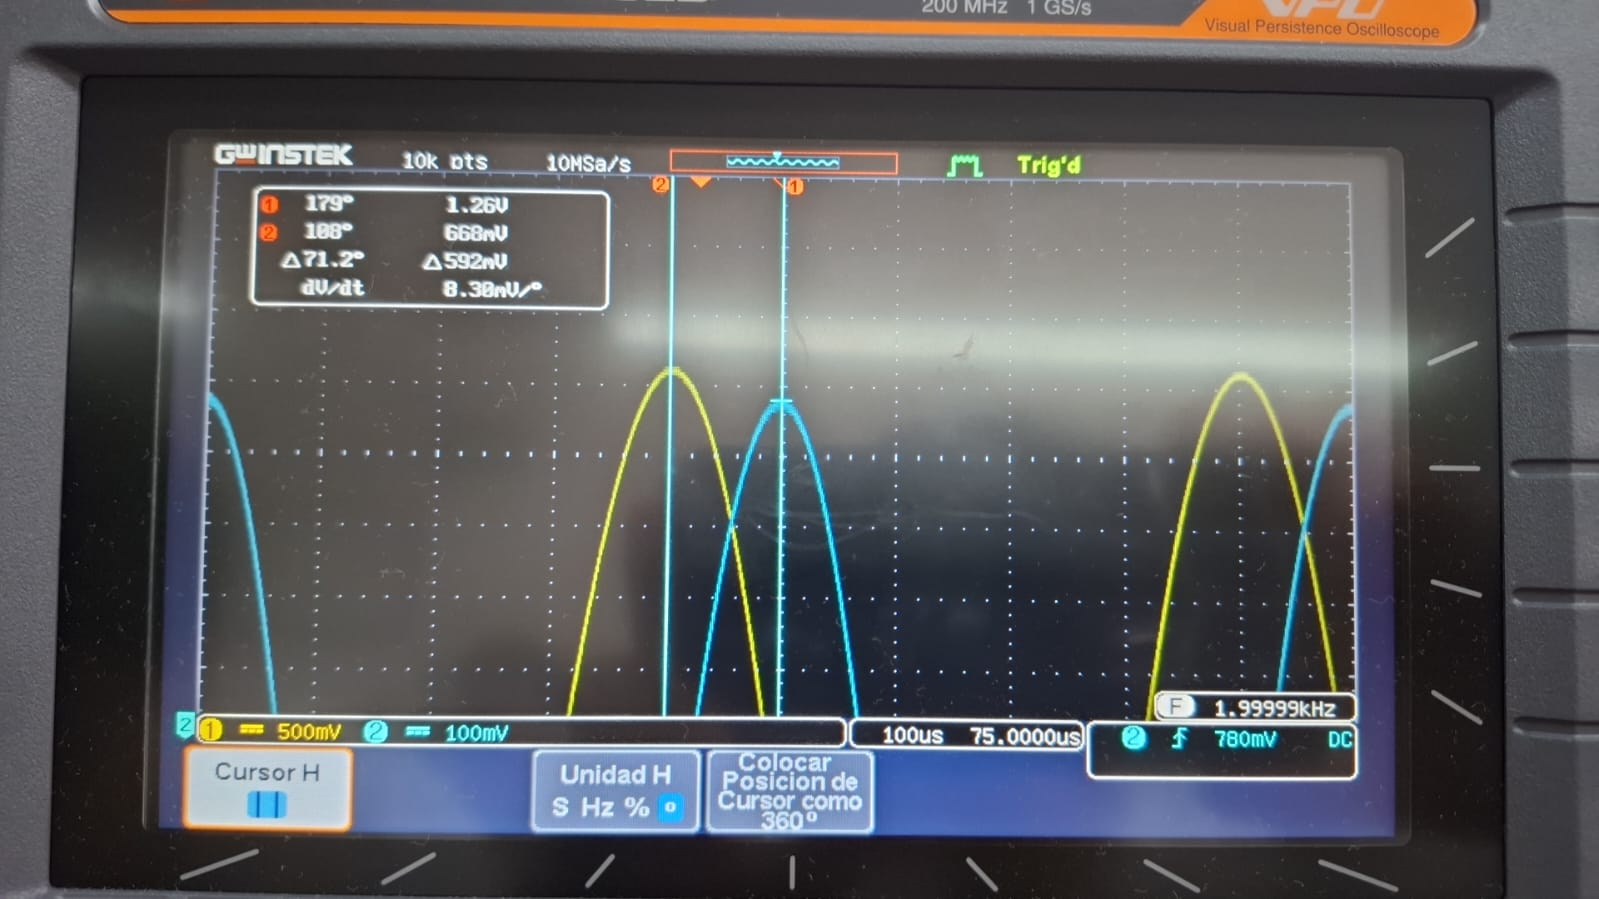
\includegraphics[width=0.7\textwidth]{e2_1.jpg}
	\caption{Osciloscopio circuito RL}
\end{figure}

\subsubsection*{Medidas prácticas}

\begin{itemize}
	\item \textbf{Ángulo de desfasamiento:} \(\Theta = \frac{1 [cuadro]\cdot (360°)}{5 [cuadros]} = 72°\)
	\item \textbf{Desfasamiento medido con cursor del osciloscopio:} \(71.2°\)
\end{itemize}

\subsection*{Cálculo de \(L\) con cuadros}

Despejamos \(L\):

\[
L = \frac{R_{eq}}{\omega} \cdot \tan(\Theta)
\]

Sustituimos para obtener \(L\):

\[
L = \frac{200 \Omega + 72.7 \Omega + 50 \Omega}{4000 \pi \, [\frac{rad}{s}]} \cdot \tan(72°) \approx 78.9 mH
\]

\begin{tcolorbox}[colback=mygray, colframe=LimeGreen, boxrule=0.7pt, arc=2pt, boxsep=1pt, left=2pt, right=2pt, top=2pt, bottom=2pt, title=Medida del inductor con cuadros]
\(L \approx 78.9 mH\)
\end{tcolorbox}

\textbf{Error porcentual:}

\[
\text{Error} = \left| \frac{L_{teorico} - L_{practico}}{L_{teorico}} \right| \cdot 100\%
\]
\[
\text{Error} = \left| \frac{78.9 mH - 72 mH}{72 mH} \right| \cdot 100\% = 9.58\%
\]

\begin{tcolorbox}[colback=mygray, colframe=LimeGreen, boxrule=0.7pt, arc=2pt, boxsep=1pt, left=2pt, right=2pt, top=2pt, bottom=2pt, title=Error porcentual]
\(E\% = 9.58\%\)
\end{tcolorbox}

\subsection*{Cálculo de \(L\) con cursor}

Sustituimos para obtener \(L\):

\[
L = \frac{200 \Omega + 72.7 \Omega + 50 \Omega}{4000 \pi \, [\frac{rad}{s}]} \cdot \tan(71.2°) \approx 75.3 mH
\]

\begin{tcolorbox}[colback=mygray, colframe=LimeGreen, boxrule=0.7pt, arc=2pt, boxsep=1pt, left=2pt, right=2pt, top=2pt, bottom=2pt, title=Medida del inductor con cursor]
\(L \approx 75.3 mH\)
\end{tcolorbox}

\textbf{Error porcentual:}

\[\text{Error} = \left| \frac{75.3 mH - 72 mH}{72 mH} \right| \cdot 100\% = 4.58\%\]

\subsection*{Experimento 2. Circuito RC}

\begin{figure}[H]
	\centering
	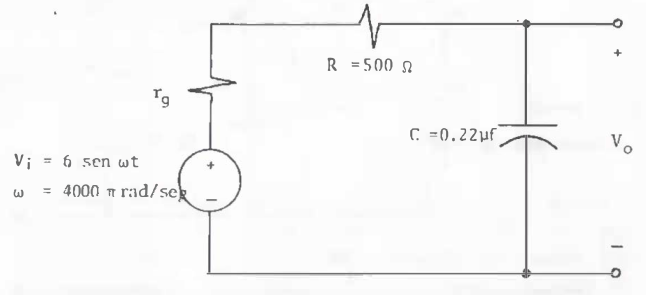
\includegraphics[width=0.6\textwidth]{figure_2.png}
	\caption{Circuito RC}
\end{figure}

\subsubsection*{Función de Transferencia}

\[H(s) = \frac{1}{1+sR_{eq}C}\]

\[H(j\omega) = \frac{1}{1+j\omega R_{eq}C}\]

\subsubsection*{Obtención de ángulo de fase}

\[\Theta_Y = \angle Y(j\omega)\]

\[\Theta_X = \angle X(j\omega)\]

\[\Theta_Y = \tan^{-1}\left(\frac{\text{Im}(Y(j\omega))}{\text{Re}(Y(j\omega))}\right)\]

\[\Theta_X = \tan^{-1}\left(\frac{\text{Im}(X(j\omega))}{\text{Re}(X(j\omega))}\right)\]

\[\Theta_H = \Theta_Y - \Theta_X\]

\[\Theta_H = \tan^{-1}\left(R_{eq}C\omega\right)\]

\[\Theta_H = \tan^{-1}\left((50\Omega +500[\Omega] )0.22[\mu F] 4000 \pi \, \left[\frac{rad}{s} \right] \right)\]

\[\Theta_H = 56.66°\]

\subsubsection*{Magnitud de la señal}

\[
|H(j\omega)| = \frac{1}{\sqrt{1 + (\omega R_{eq} C)^2}}
\]

\subsubsection*{Datos de Practica}

\begin{itemize}
	\item \textbf{Señal de entrada:} \(6 sen (\omega t)\)
	\item \textbf{\(\omega\):} \(4000 \pi \, rad/s\)
	\item \textbf{Frecuencia:} \(f = 2 kHz\)
	\item \textbf{Resistencia de la fuente:} \(50 \omega\)
	\item \textbf{Capacitancia:} \(C =  0.22 \mu F\)
	\item \textbf{Resistencia:} \(R = 500 \Omega\)
\end{itemize}

\begin{figure}[H]
	\centering
	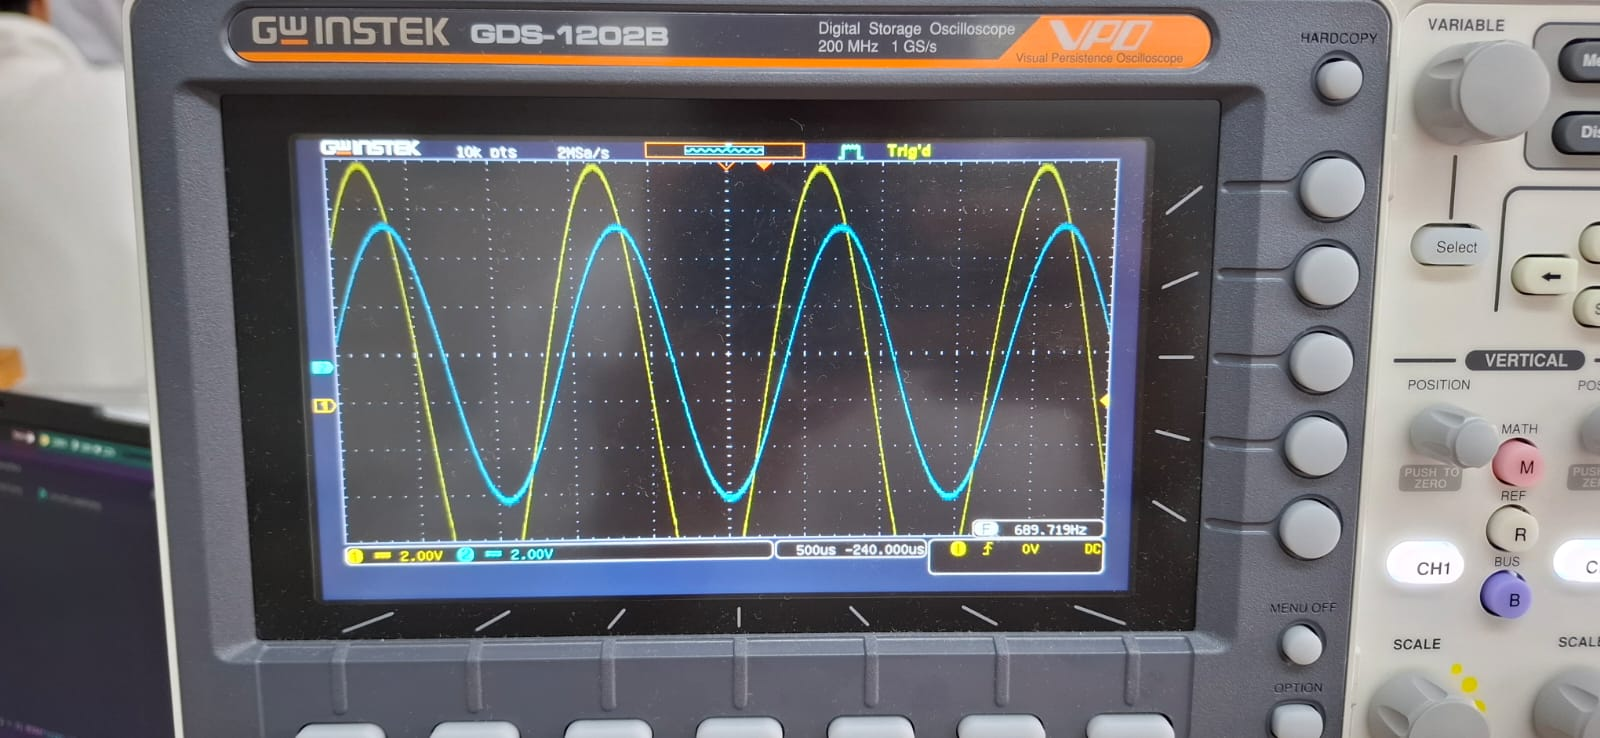
\includegraphics[width=0.7\textwidth]{e2.jpg}
	\caption{Osciloscopio circuito RC}
\end{figure}

\subsubsection*{Medidas prácticas}

\begin{itemize}
	\item \textbf{Desfasamiento medido con cursor del osciloscopio:} \(56.1°\)
\end{itemize}

Despejamos \(C\):

\[
C = \frac{1}{\omega R_{eq}} \cdot \tan(\Theta)
\]

Sustituimos para obtener \(C\):

\[
C = \frac{1}{500 \Omega + 50 \Omega} \cdot \tan(56.1°) \approx 0.21 [\mu F]
\]

\begin{tcolorbox}[colback=mygray, colframe=LimeGreen, boxrule=0.7pt, arc=2pt, boxsep=1pt, left=2pt, right=2pt, top=2pt, bottom=2pt, title=Medida del capacitor con cursor]
\(C \approx 0.21 [\mu F]\)
\end{tcolorbox}

\textbf{Error porcentual:}

\[
\text{Error} = \left| \frac{C_{teorico} - C_{practico}}{C_{teorico}} \right| \cdot 100\%
\]
\[
\text{Error} = \left| \frac{0.22 [\mu F] - 0.21 [\mu F]}{0.22 [\mu F]} \right| \cdot 100\% = 4.54\%
\]

\begin{tcolorbox}[colback=mygray, colframe=LimeGreen, boxrule=0.7pt, arc=2pt, boxsep=1pt, left=2pt, right=2pt, top=2pt, bottom=2pt, title=Error porcentual]
\(E\% = 4.54\%\)
\end{tcolorbox}

\subsection*{Experimento 3.Circuito RC invertido}

\subsubsection*{Ángulo de fase}

\[
\Theta_H = \tan^{-1}\left(\frac{1}{R_{eq}C\omega}\right)
\]

\[
\Theta_H = \tan^{-1}\left(\frac{1}{(50\Omega + 500\Omega)0.22[\mu F] 4000 \pi \, \left[\frac{rad}{s} \right]}\right)
\]

\[
\Theta_H = 33.33°
\]

\subsubsection*{Datos de Practica}

\begin{itemize}
	\item \textbf{Señal de entrada:} \(6 sen (\omega t)\)
	\item \textbf{\(\omega\):} \(4000 \pi \, rad/s\)
	\item \textbf{Frecuencia:} \(f = 2 kHz\)
	\item \textbf{Resistencia de la fuente:} \(50 \Omega\)
	\item \textbf{Capacitancia:} \(C =  0.22 \mu F\)
	\item \textbf{Resistencia:} \(R = 500 \Omega\)
\end{itemize}

\subsubsection*{Medidas prácticas}

\begin{itemize}
	\item \textbf{Desfasamiento medido con cursor del osciloscopio:} \(36.8°\)
\end{itemize}

Despejamos \(C\):

\[
C = \frac{1}{R_{eq}\cdot \omega \cdot \tan(\Theta_H)}
\]

Sustituimos para obtener \(C\):

\[
C = \frac{1}{(50\Omega + 500\Omega) 4000 \pi \, \left[\frac{rad}{s} \right]\cdot \tan(36.8°)} \approx 0.19[\mu F]
\]

\begin{tcolorbox}[colback=mygray, colframe=LimeGreen, boxrule=0.7pt, arc=2pt, boxsep=1pt, left=2pt, right=2pt, top=2pt, bottom=2pt, title=Medida del capacitor con cursor]
\(C \approx 0.19 [\mu F]\)
\end{tcolorbox}

\textbf{Error porcentual:}

\[
\text{Error} = \left| \frac{C_{teorico} - C_{practico}}{C_{teorico}} \right| \cdot 100\%
\]
\[
\text{Error} = \left| \frac{0.22 [\mu F] - 0.19 [\mu F]}{0.22 [\mu F]} \right| \cdot 100\% = 15.78\%
\]

\begin{tcolorbox}[colback=mygray, colframe=LimeGreen, boxrule=0.7pt, arc=2pt, boxsep=1pt, left=2pt, right=2pt, top=2pt, bottom=2pt, title=Error porcentual]
\(E\% = 15.78\%\)
\end{tcolorbox}

\subsubsection*{Observacion entre circuitos RC}

A diferencia del circuito anterior al colocar el capacitor primero vemos que ahora está adelanta con respecto a la señal de entrada.

\subsection*{Experimento 4. Circuito RLC}

\begin{figure}[H]
	\centering
	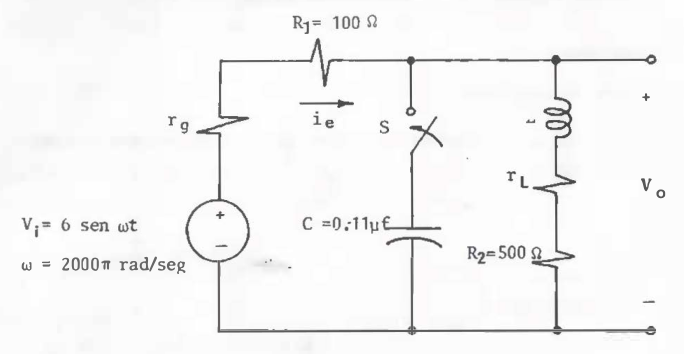
\includegraphics[width=0.6\textwidth]{figure_3.png}
	\caption{Circuito RLC}
\end{figure}

\subsubsection*{Ángulo de desfase}

\[
\Theta = \tan^{-1} \left(\frac{\omega C(r_L + R_2)}{1 -\omega LC} \right) - \tan^{-1}\left(\frac{\omega L}{r_L + R_2} \right)
\]

\[
\Theta = \tan^{-1} \left(\frac{(2000\pi)(0.11 \mu F)(72.7 \Omega + 500 \Omega)}{1 - (2000\pi)(0.11 \mu F)(72 mH)} \right) - \tan^{-1}\left(\frac{(2000\pi)(72 mH)}{72.7 \Omega + 500 \Omega} \right)
\]

\[
\Theta = 21.59° - 38.30° = -16.71°
\]

\subsubsection*{Datos de Practica}

\begin{itemize}
	\item \textbf{Señal de entrada:} \(6 sen (\omega t)\)
	\item \textbf{\(\omega\):} \(2000 \pi \, rad/s\)
	\item \textbf{Frecuencia:} \(f = 1 kHz\)
	\item \textbf{Resistencia de la fuente:} \(50 \Omega\)
	\item \textbf{Capacitancia:} \(C =  0.11 \mu F\)
	\item \textbf{Inductancia:} \(L =  72 mH\)
	\item \textbf{Resistencia del inductor:} \(R_L = 72.7 \Omega\)
	\item \textbf{Resistencia:} \(R_1 = 100 \Omega\)
	\item \textbf{Resistencia:} \(R_2 = 500 \Omega\)
\end{itemize}

En este ultimo expermiento no se midió nada ya que los osciloscopios proporcionaban muco ruido en el canal 2 pero logramos observar que al invertir la señal de salida era igual a la de entrada.

\begin{figure}[H]
	\centering
	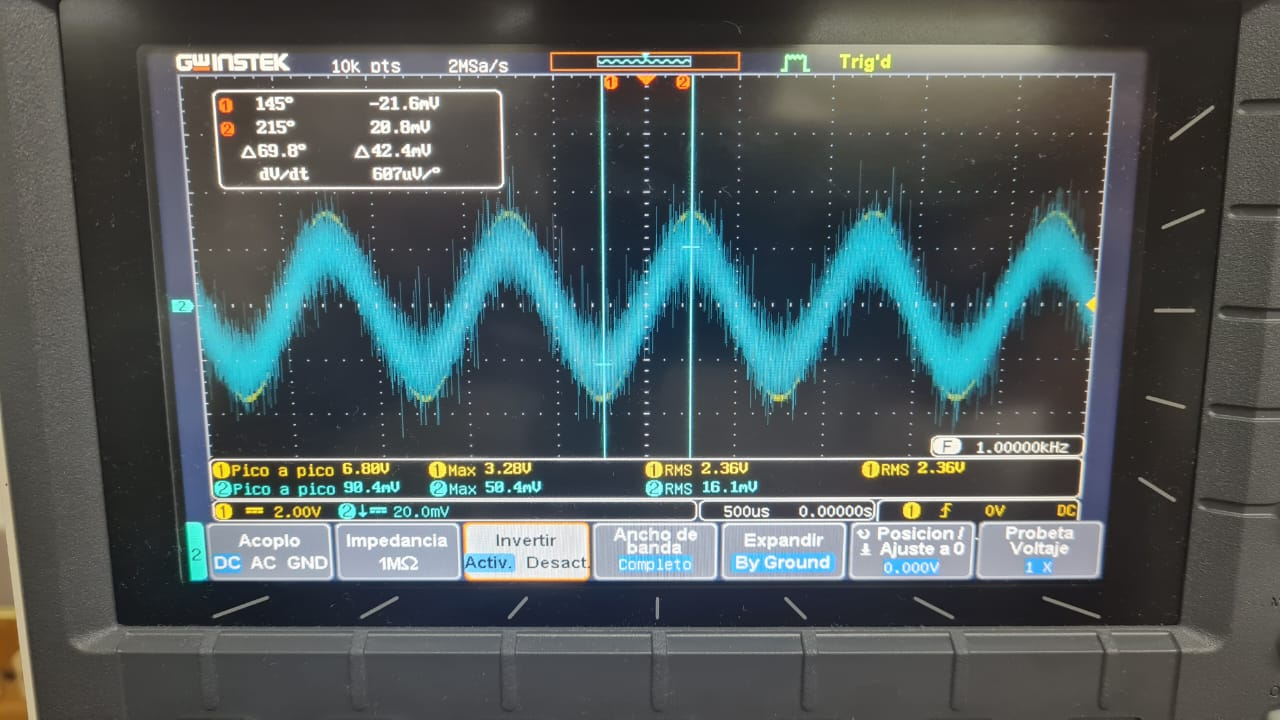
\includegraphics[width=0.7\textwidth]{e4.jpg}
	\caption{Osciloscopio circuito RLC}
\end{figure}

\subsection*{Conclusiones}

\subsubsection*{Tepal Brinseño Hansel Yael}

Pudimos observar que en el circuito RL la señal de salida se atrasa respecto a la entrada debido a la presencia del inductor, el cual se opone a los cambios de corriente. Este atraso fue de aproximadamente 71.2°, confirmando la naturaleza inductiva del circuito. En los circuitos RC se vió la diferencia entre las configuraciones cuando se mide la salida en el capacitor y cuando se invierte. Los errores porcentuales obtenidos (4.58\% para el inductor y 4.54\% para el capacitor en configuración pasa-bajos) validan la precisión del método fasorial para el análisis de circuitos en régimen senoidal permanente.

\subsubsection*{Ugartechea González Luis Antonio}

El análisis fasorial demostró ser una herramienta eficaz para predecir y verificar el comportamiento de circuitos lineales ante señales sinusoidales. Los inductores introducen un atraso de fase en la señal de salida debido a su impedancia reactiva positiva, lo que provoca que la corriente se atrase respecto al voltaje aplicado, mientras que los capacitores pueden causar adelanto o atraso dependiendo de su configuración. En configuración pasa-bajos (RC) la señal se atrasa, y en configuración pasa-altos (CR) la señal se adelanta, debido a la impedancia reactiva negativa del capacitor. La precisión de las mediciones mejoró significativamente al utilizar los cursores del osciloscopio en lugar del método de conteo de cuadros, reduciendo el error del 9.58\% al 4.58\% en el caso del inductor.



% \section{Bibliography}

% \begin{biblio}
% 	%for: https://www.poli.edu.co/blog/poliverso/diseno-digital-que-es
% 	\item \textit{Diseño digital: qué es y por qué es importante.} (2021, August 26). Poliverso. Retrieved October 16, 2024, from: \textcolor{blue}{\underline{\url{https://www.poli.edu.co/blog/poliverso/diseno-digital-que-es}}}
% 	%for: https://www.sky6cancun.com/marketing/diseno-grafico/diseno-digital-que-es-y-para-que-sirve/
% 	\item \textit{Diseño digital: qué es y para qué sirve.} (2021, August 26). Sky6Cancún. Retrieved October 16, 2024, from: \textcolor{blue}{\underline{\url{https://www.sky6cancun.com/marketing/diseno-grafico/}}}
% \end{biblio}

\end{document}
